\documentclass[12pt,a4paper]{article}

% Packages
\usepackage[utf8]{inputenc}
\usepackage[T1]{fontenc}
\usepackage{geometry}
\usepackage{graphicx}
\usepackage{amsmath}
\usepackage{amsfonts}
\usepackage{amssymb}
\usepackage{booktabs}
\usepackage{hyperref}
\usepackage{float}
\usepackage{caption}
\usepackage{subcaption}
\usepackage{xcolor}
\usepackage{listings}
\usepackage{fancyhdr}
\usepackage{titlesec}
\usepackage{tocloft}

% Page geometry
\geometry{margin=1in}

% Header/Footer
\pagestyle{fancy}
\fancyhf{}
\rhead{Loan Approval Prediction}
\lhead{Mid-Semester Project}
\cfoot{\thepage}

% Hyperref setup
\hypersetup{
    colorlinks=true,
    linkcolor=blue,
    filecolor=magenta,
    urlcolor=cyan,
}

% Title formatting
\titleformat{\section}{\Large\bfseries}{\thesection}{1em}{}
\titleformat{\subsection}{\large\bfseries}{\thesubsection}{1em}{}

% Code listing style
\lstset{
    basicstyle=\ttfamily\small,
    breaklines=true,
    frame=single,
    backgroundcolor=\color{gray!10}
}

\begin{document}

% Title Page
\begin{titlepage}
    \centering
    \vspace*{2cm}
    
    {\Huge\bfseries Loan Approval Prediction System\par}
    \vspace{0.5cm}
    {\Large Using Machine Learning and Deep Learning\par}
    
    \vspace{2cm}
    
    {\large Mid-Semester AI/ML Project Report\par}
    
    \vspace{3cm}
    
    {\Large\bfseries Author\par}
    \vspace{0.3cm}
    {\large Mitul Bhatia\par}
    
    \vspace{2cm}
    
    {\large\bfseries GitHub Repository\par}
    \vspace{0.3cm}
    {\url{https://github.com/mitul-bhatia/GEN_AI_LOAN_APPROVAL}\par}
    
    \vfill
    
    {\large February 2026\par}
\end{titlepage}

% Table of Contents
\tableofcontents
\newpage

% Abstract
\begin{abstract}
This report presents a comprehensive machine learning approach to predict loan approval decisions. Using a dataset of 50,000 loan applications with 20 features, we develop and evaluate multiple classification models. Our analysis begins with Logistic Regression as a principled baseline, achieving 86.42\% accuracy and 0.944 ROC-AUC. The report documents our complete methodology including exploratory data analysis, feature engineering, model development with mathematical foundations, and thorough evaluation. Key findings reveal that product type and loan intent are stronger predictors than traditional credit metrics, with Credit Card products showing 33x higher approval odds compared to baseline.
\end{abstract}

\newpage

% Section 1: Introduction
\section{Introduction}

\subsection{Problem Statement}

Loan approval is a critical decision in financial institutions, balancing risk management with customer acquisition. Manual assessment is time-consuming, inconsistent, and cannot scale to handle millions of applications. This project develops an automated loan approval prediction system using machine learning.

\subsection{Objectives}

\begin{enumerate}
    \item Develop accurate classification models to predict loan approval
    \item Identify key factors influencing approval decisions
    \item Compare traditional ML algorithms with deep learning approaches
    \item Deploy a production-ready web application
\end{enumerate}

\subsection{Scope}

This project implements:
\begin{itemize}
    \item Exploratory Data Analysis (EDA) with comprehensive visualizations
    \item Traditional ML models: Logistic Regression, Decision Trees, Random Forest, XGBoost
    \item Deep Learning model using Keras
    \item Streamlit web application for real-time predictions
\end{itemize}

\newpage

% Section 2: Dataset
\section{Dataset Description}

\subsection{Overview}

The Loan Approval Dataset 2025 contains \textbf{50,000 loan applications} with \textbf{20 features}. The dataset is clean with no missing values.

\subsection{Features}

\begin{table}[H]
\centering
\caption{Dataset Features}
\begin{tabular}{lll}
\toprule
\textbf{Feature} & \textbf{Type} & \textbf{Description} \\
\midrule
customer\_id & String & Unique identifier (dropped) \\
age & Integer & Applicant age (18-70) \\
occupation\_status & Categorical & Employed/Self-Employed/Student \\
years\_employed & Float & Years of employment \\
annual\_income & Integer & Annual income (15,000-250,000) \\
credit\_score & Integer & Credit score (300-850) \\
credit\_history\_years & Float & Length of credit history \\
savings\_assets & Integer & Savings and assets value \\
current\_debt & Integer & Current debt amount \\
defaults\_on\_file & Integer & Number of past defaults \\
delinquencies\_last\_2yrs & Integer & Recent payment delinquencies \\
derogatory\_marks & Integer & Negative credit marks \\
product\_type & Categorical & Credit Card/Personal Loan/Line of Credit \\
loan\_intent & Categorical & Purpose of loan \\
loan\_amount & Integer & Requested loan amount \\
interest\_rate & Float & Interest rate offered \\
debt\_to\_income\_ratio & Float & DTI ratio \\
loan\_to\_income\_ratio & Float & LTI ratio \\
payment\_to\_income\_ratio & Float & PTI ratio \\
\textbf{loan\_status} & \textbf{Binary} & \textbf{Target: 0=Rejected, 1=Approved} \\
\bottomrule
\end{tabular}
\end{table}

\subsection{Target Variable Distribution}

The target variable is reasonably balanced:
\begin{itemize}
    \item \textbf{Approved (1)}: 27,523 applications (55.05\%)
    \item \textbf{Rejected (0)}: 22,477 applications (44.95\%)
\end{itemize}

This balance means we do not require oversampling techniques like SMOTE.

\begin{figure}[H]
    \centering
    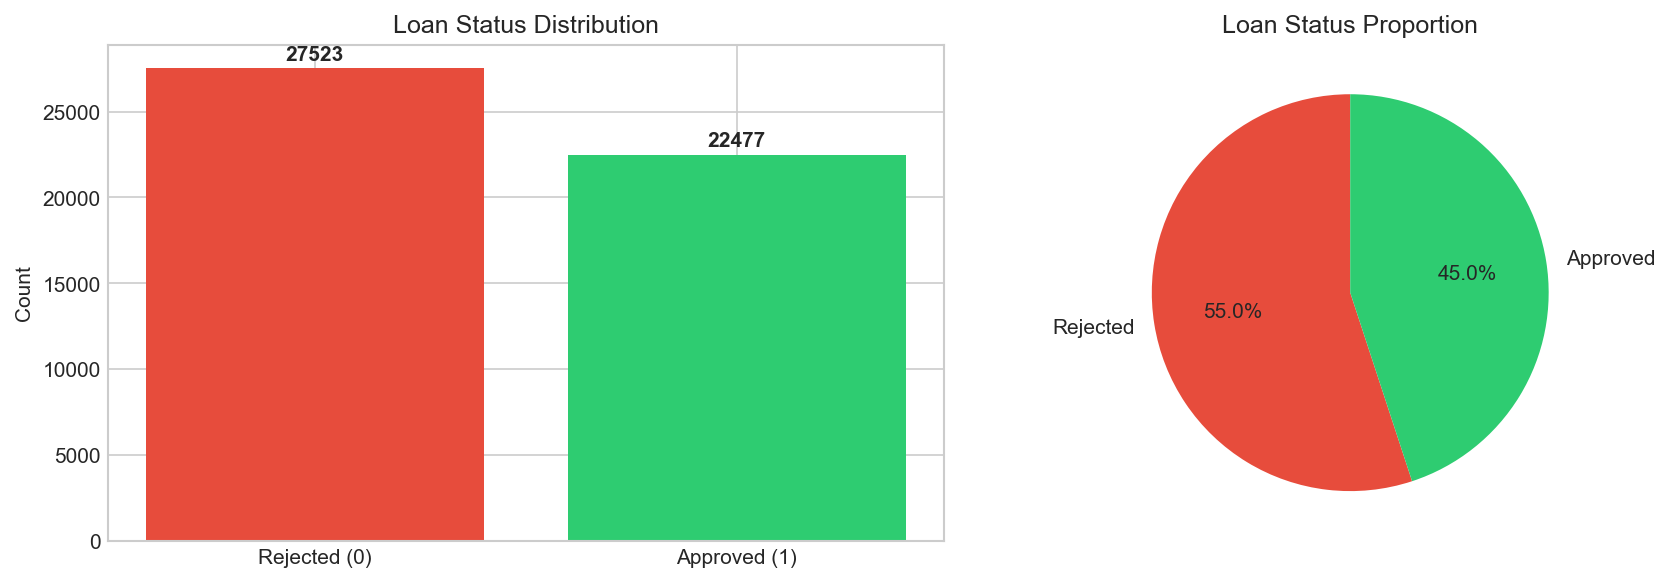
\includegraphics[width=0.9\textwidth]{target_distribution.png}
    \caption{Target Variable Distribution}
    \label{fig:target_dist}
\end{figure}

\newpage

% Section 3: EDA
\section{Exploratory Data Analysis}

\subsection{Numerical Features Distribution}

Analysis of numerical features reveals several patterns:

\begin{itemize}
    \item \textbf{Age}: Ranges from 18-70, with approved applicants skewing slightly older
    \item \textbf{Credit Score}: Strong separator between approved (higher) and rejected (lower) applications
    \item \textbf{Annual Income}: Right-skewed distribution; approved applicants have higher median income
    \item \textbf{Interest Rate}: Higher rates correlate with rejection
\end{itemize}

\begin{figure}[H]
    \centering
    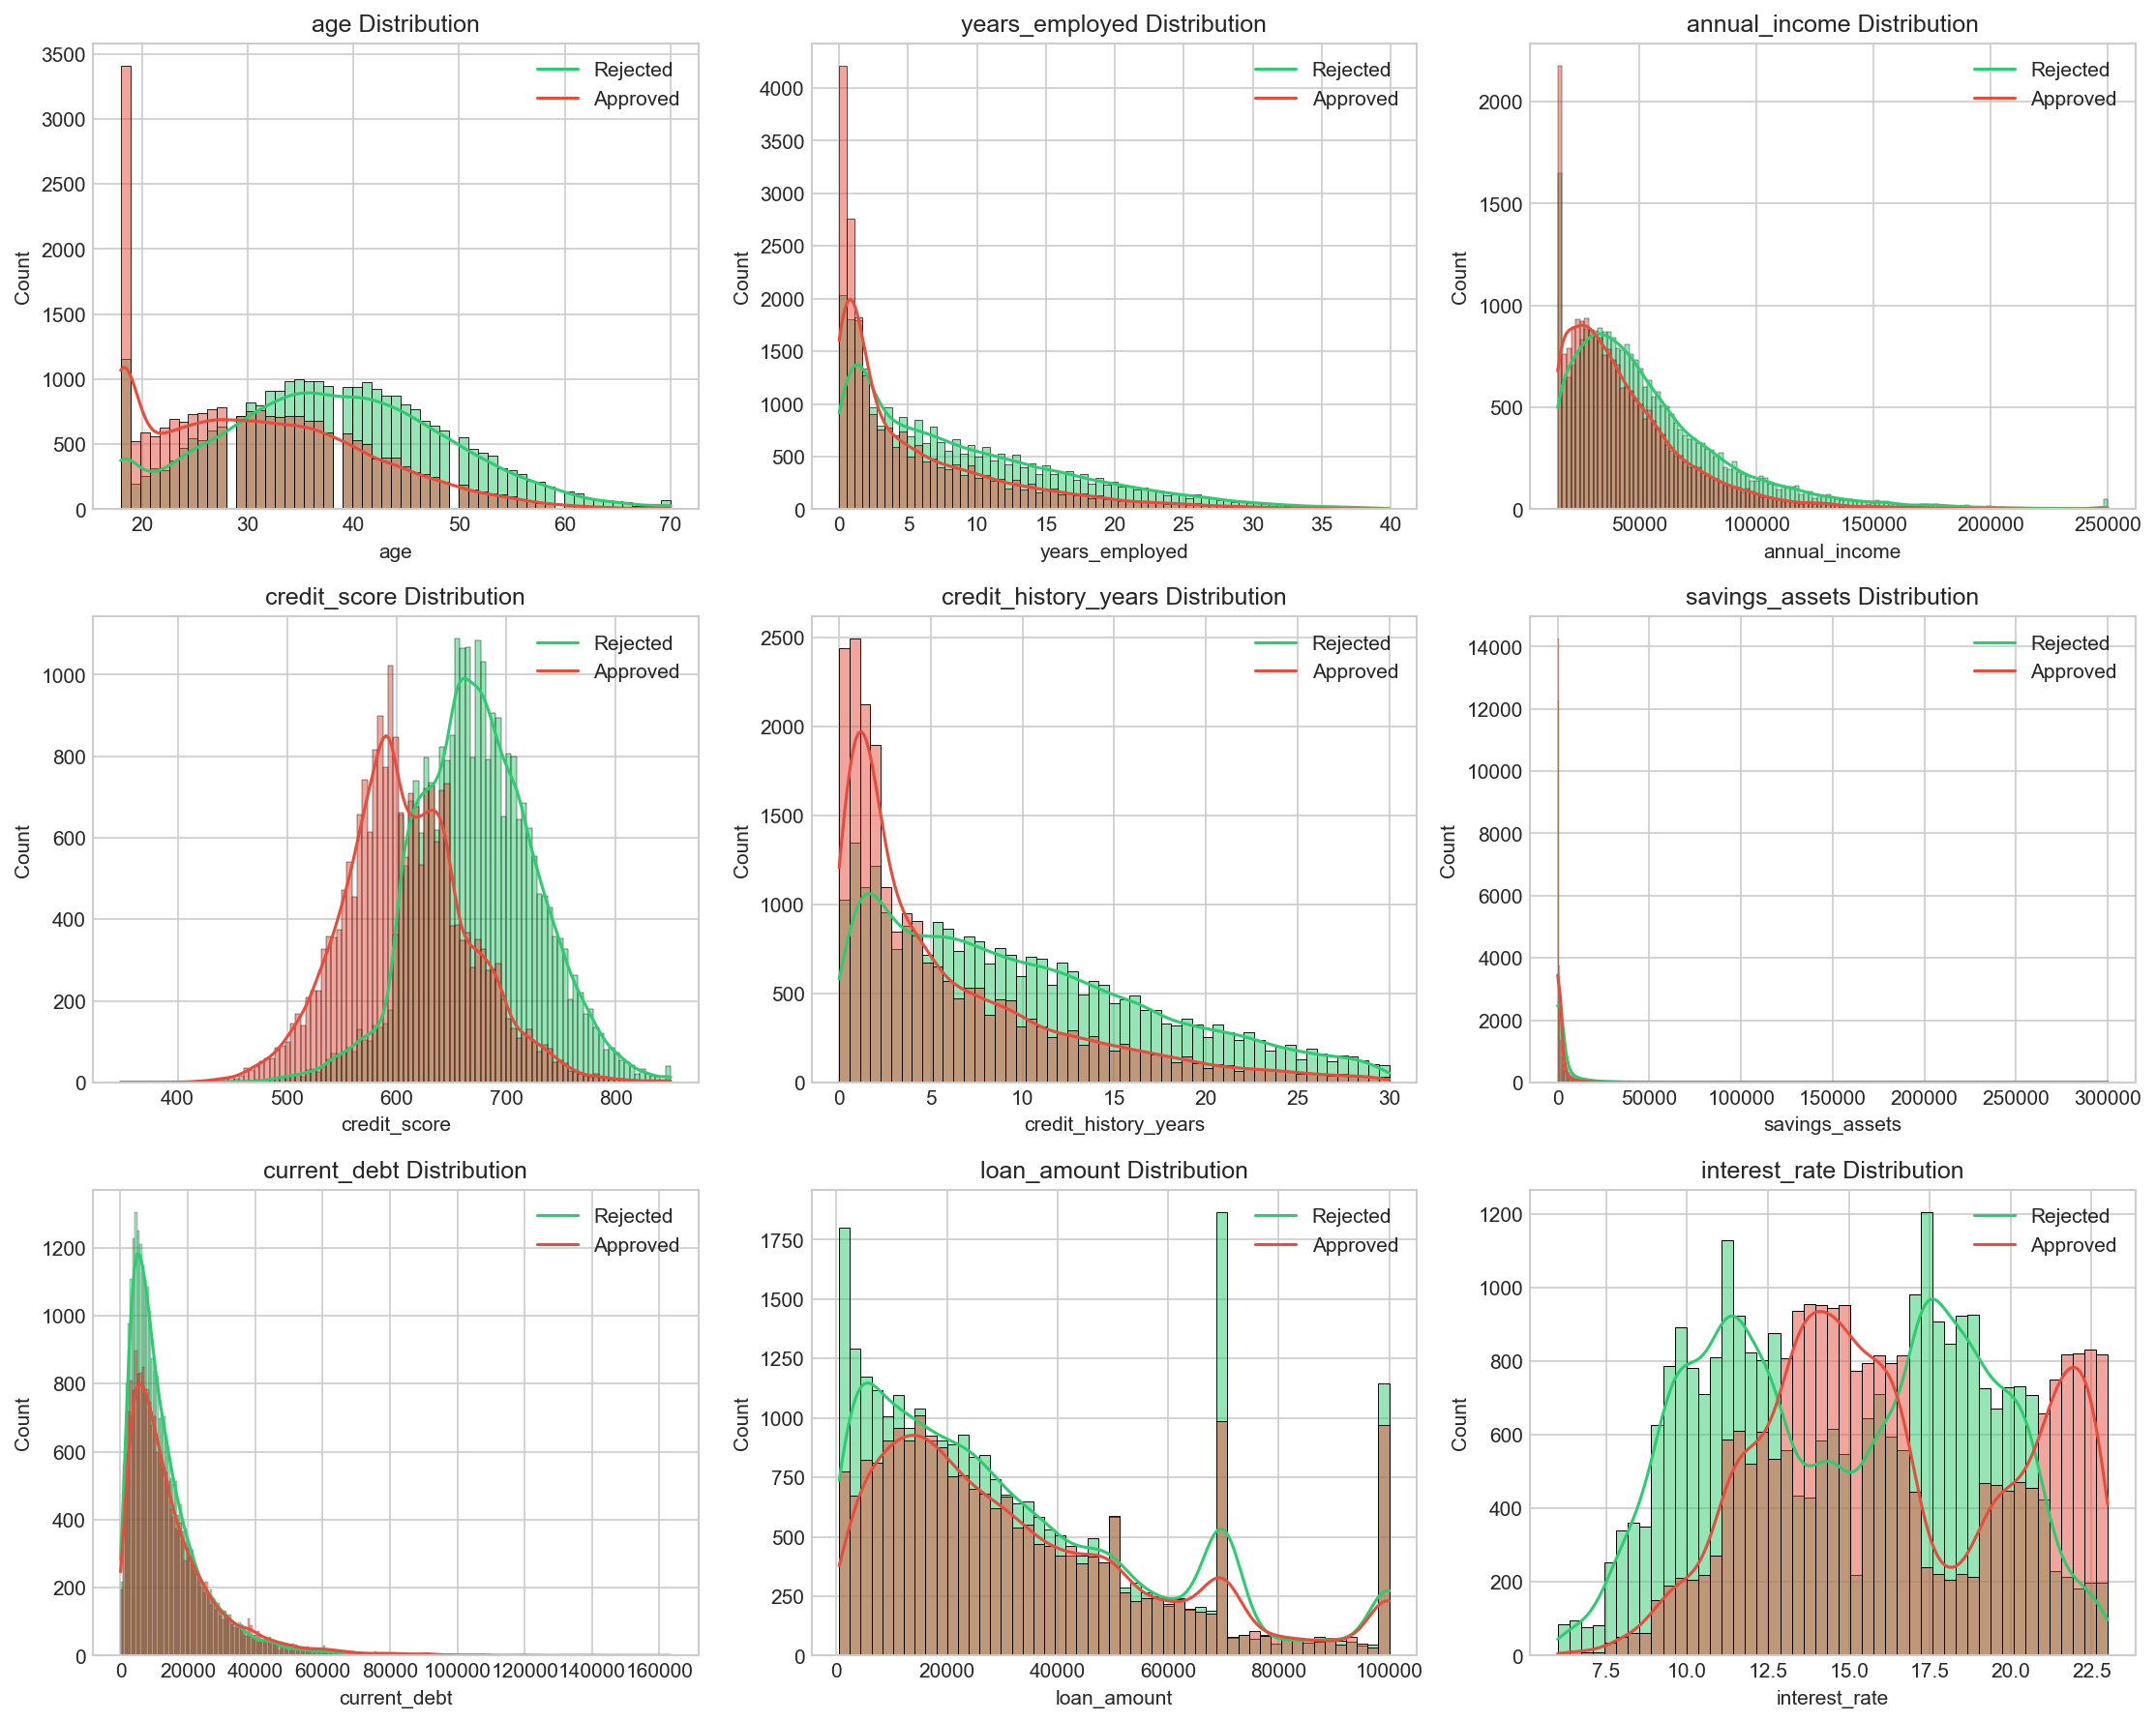
\includegraphics[width=\textwidth]{numerical_distributions.png}
    \caption{Numerical Features Distribution by Loan Status}
    \label{fig:num_dist}
\end{figure}

\subsection{Categorical Features Analysis}

Approval rates vary significantly across categorical features:

\begin{table}[H]
\centering
\caption{Approval Rates by Category}
\begin{tabular}{llc}
\toprule
\textbf{Feature} & \textbf{Category} & \textbf{Approval Rate} \\
\midrule
\multirow{3}{*}{Occupation Status} & Self-Employed & 57\% \\
 & Student & 56\% \\
 & Employed & 54\% \\
\midrule
\multirow{3}{*}{Product Type} & Credit Card & 61\% \\
 & Line of Credit & 53\% \\
 & Personal Loan & 48\% \\
\midrule
\multirow{6}{*}{Loan Intent} & Education & 68\% \\
 & Personal & 61\% \\
 & Home Improvement & 54\% \\
 & Medical & 53\% \\
 & Business & 44\% \\
 & Debt Consolidation & 37\% \\
\bottomrule
\end{tabular}
\end{table}

\begin{figure}[H]
    \centering
    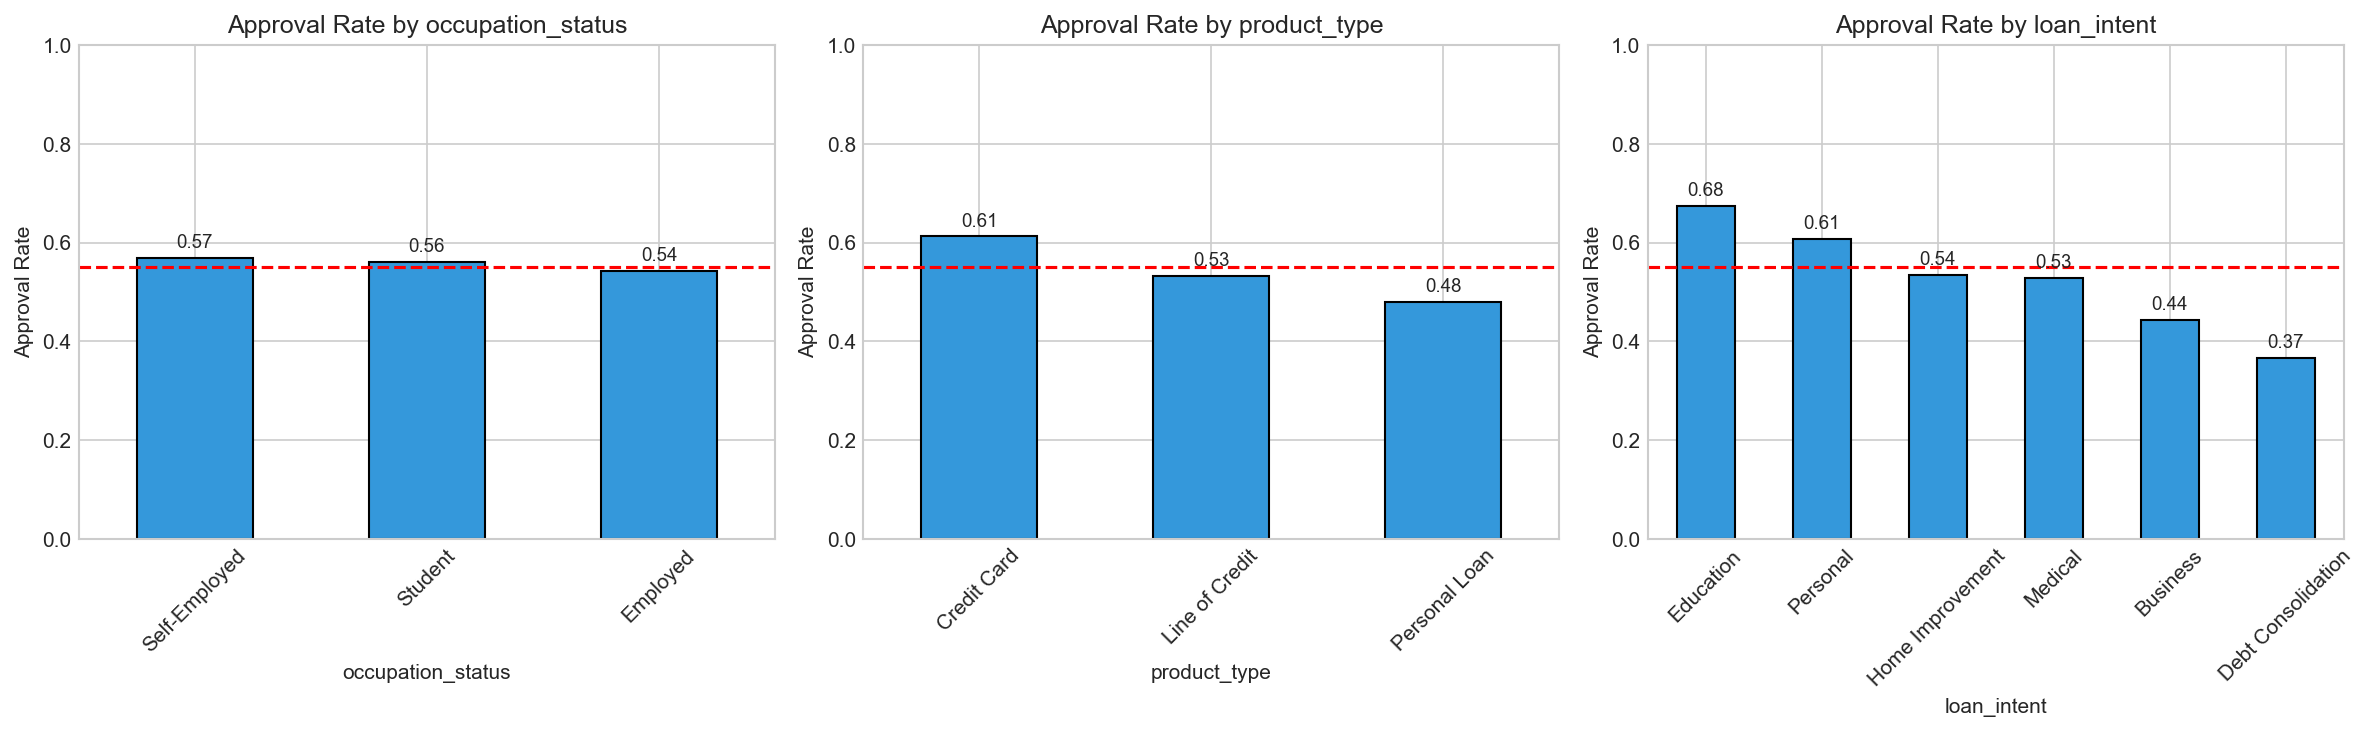
\includegraphics[width=\textwidth]{categorical_analysis.png}
    \caption{Approval Rate by Categorical Features}
    \label{fig:cat_analysis}
\end{figure}

\subsection{Correlation Analysis}

The correlation heatmap reveals:

\begin{enumerate}
    \item \textbf{Strong positive correlations with approval}: credit\_score (+0.50), age (+0.31), credit\_history\_years (+0.28)
    \item \textbf{Strong negative correlations with approval}: delinquencies\_last\_2yrs (-0.32), debt\_to\_income\_ratio (-0.32), defaults\_on\_file (-0.26)
    \item \textbf{Multicollinearity}: loan\_to\_income\_ratio and payment\_to\_income\_ratio are perfectly correlated (1.00)
\end{enumerate}

\begin{figure}[H]
    \centering
    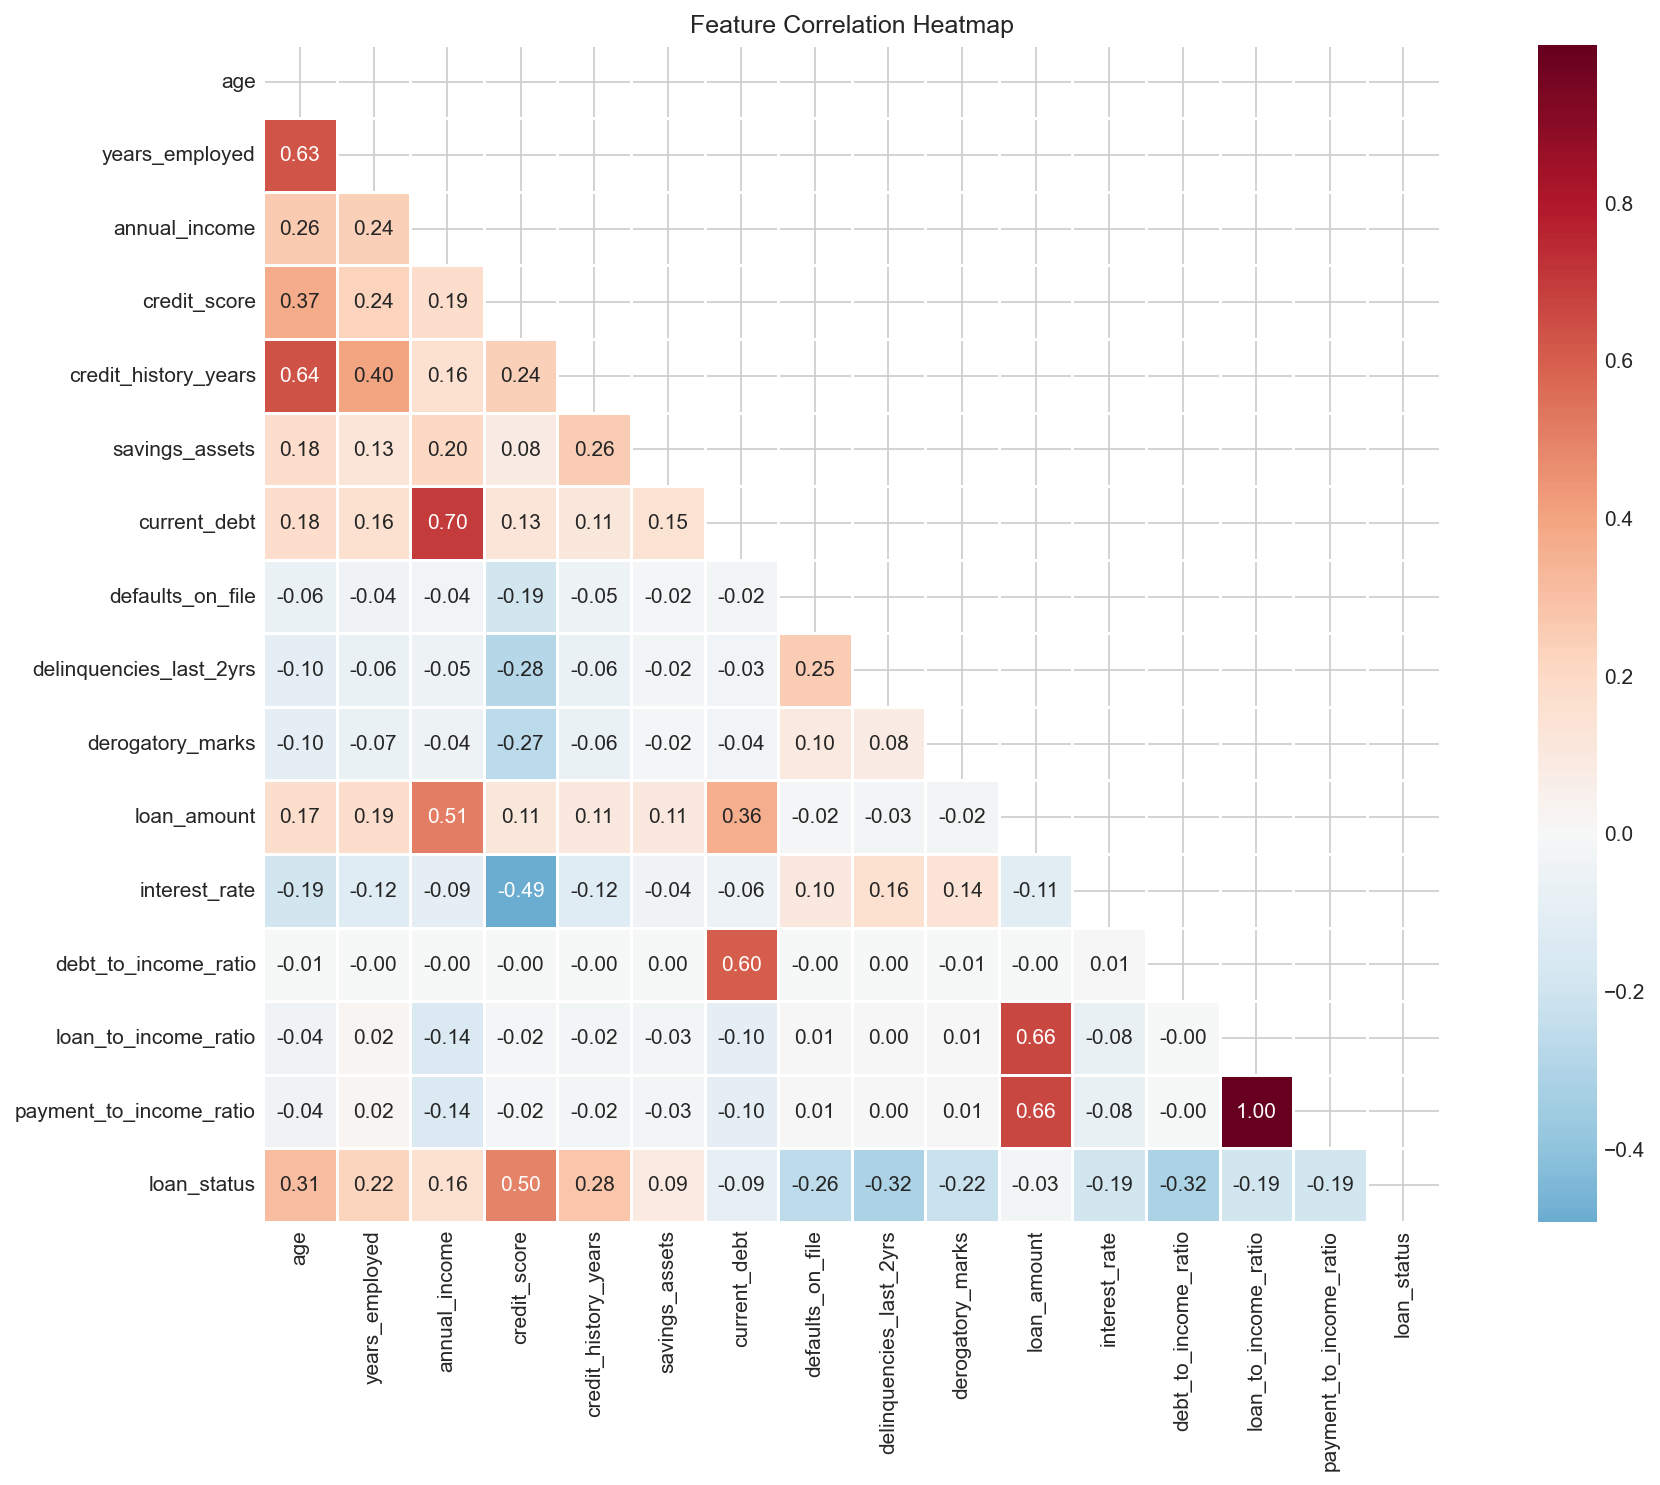
\includegraphics[width=\textwidth]{correlation_heatmap.png}
    \caption{Feature Correlation Heatmap}
    \label{fig:corr_heatmap}
\end{figure}

\begin{figure}[H]
    \centering
    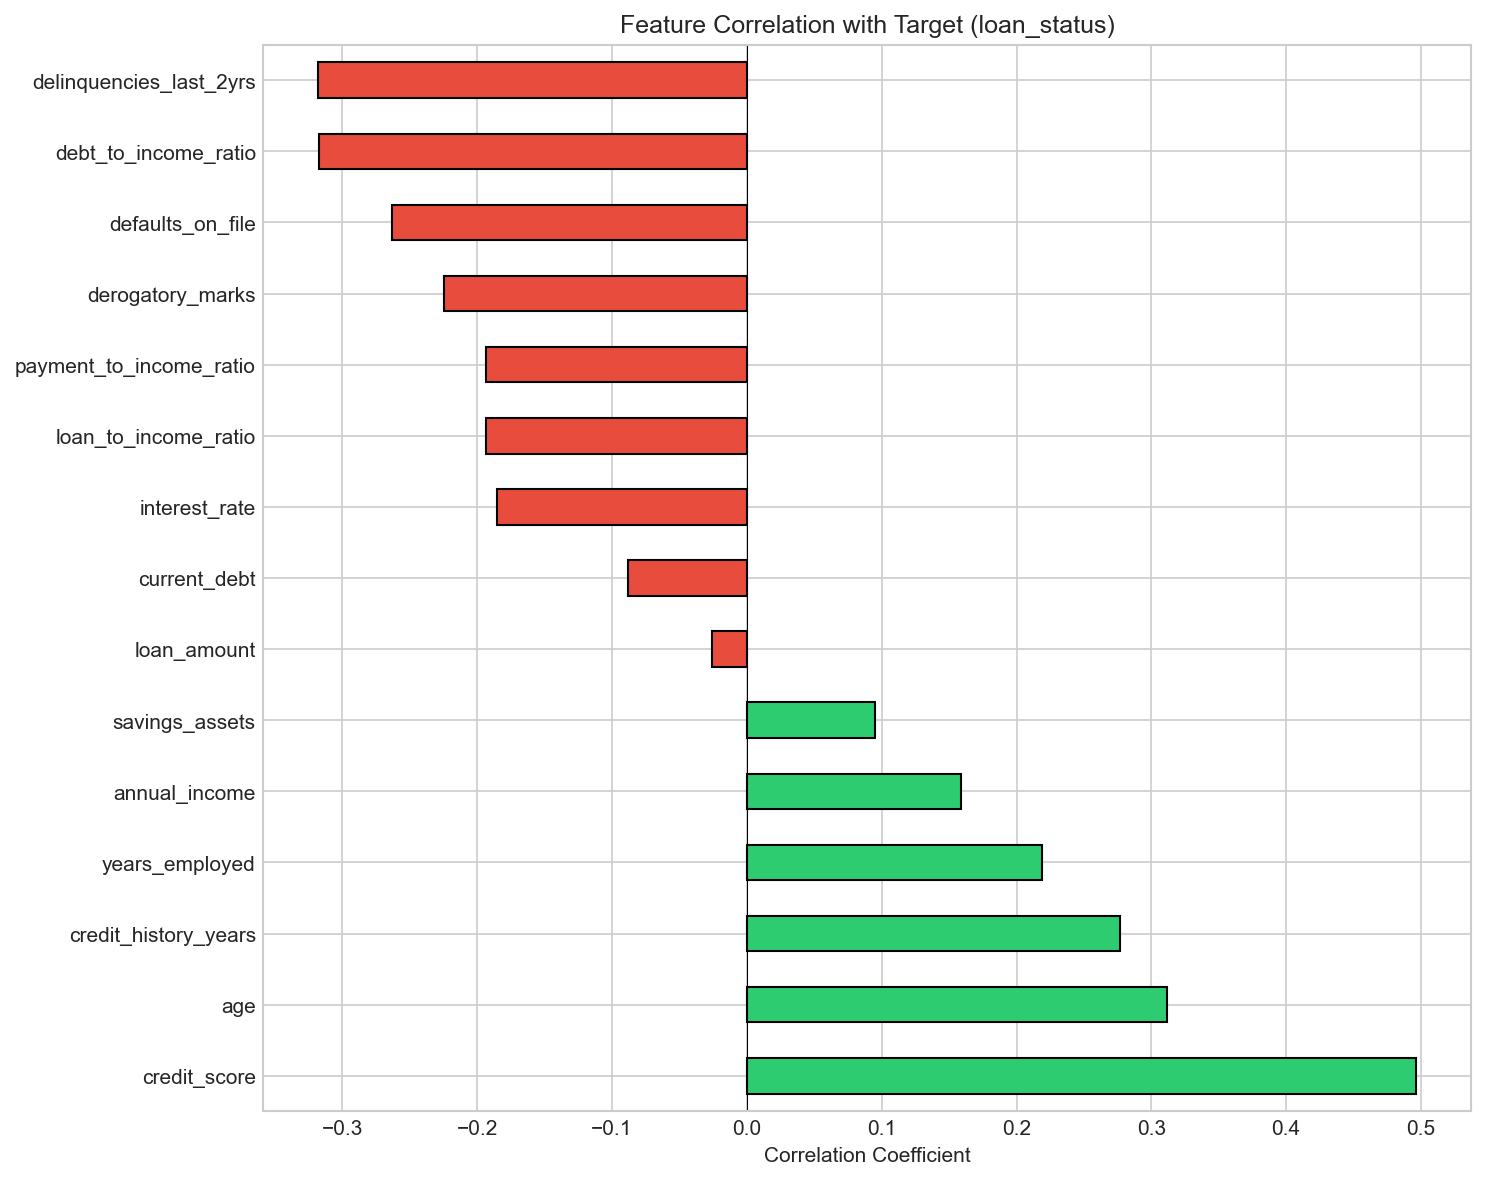
\includegraphics[width=0.85\textwidth]{target_correlation.png}
    \caption{Feature Correlation with Target Variable}
    \label{fig:target_corr}
\end{figure}

\subsection{Key Features Deep Dive}

Box plots of the most predictive features show clear separation between approved and rejected classes:

\begin{figure}[H]
    \centering
    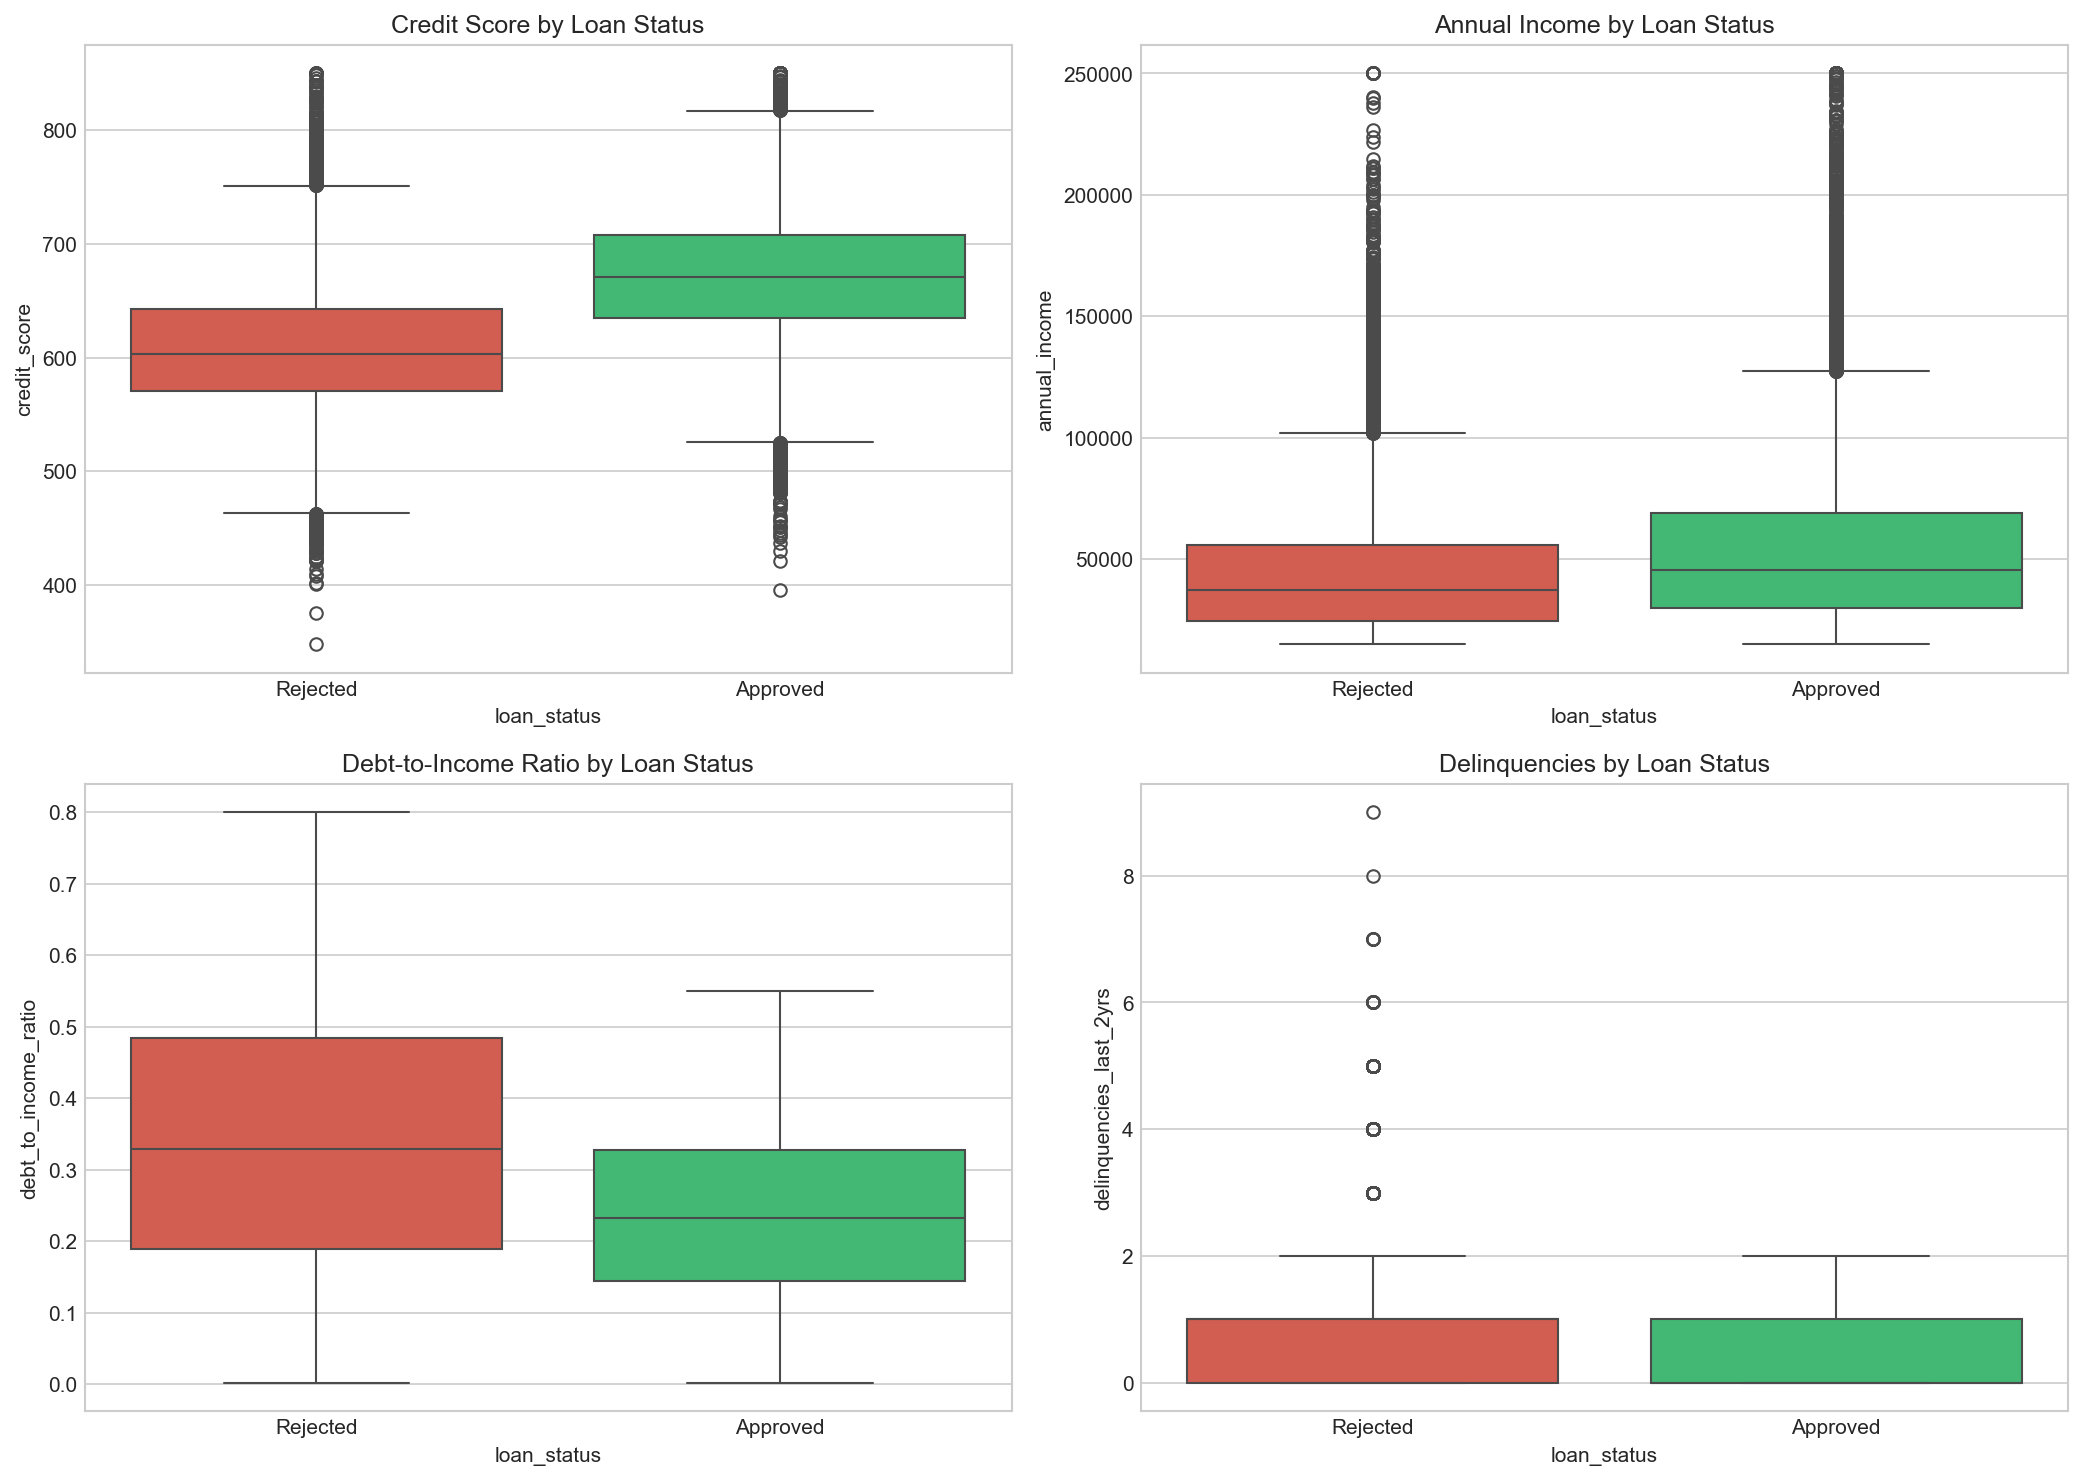
\includegraphics[width=\textwidth]{key_features_boxplot.png}
    \caption{Key Features by Loan Status}
    \label{fig:key_features}
\end{figure}

\newpage

% Section 4: Preprocessing
\section{Data Preprocessing}

\subsection{Feature Selection}

Based on EDA findings, we made the following decisions:

\textbf{Dropped Features:}
\begin{itemize}
    \item \texttt{customer\_id}: Unique identifier with no predictive value
    \item \texttt{current\_debt}: Redundant; captured by \texttt{debt\_to\_income\_ratio}
\end{itemize}

\textbf{Retained Ratios:}
We verified that \texttt{debt\_to\_income\_ratio} = \texttt{current\_debt} / \texttt{annual\_income} with 100\% match. Ratios are more meaningful than raw values as they are normalized.

\subsection{Categorical Encoding}

One-hot encoding was applied to categorical features:

\begin{itemize}
    \item \texttt{occupation\_status}: 3 categories $\rightarrow$ 3 binary features
    \item \texttt{product\_type}: 3 categories $\rightarrow$ 3 binary features
    \item \texttt{loan\_intent}: 6 categories $\rightarrow$ 6 binary features
\end{itemize}

\subsection{Feature Scaling}

StandardScaler was applied to 14 numerical features:
\[
z = \frac{x - \mu}{\sigma}
\]

This ensures all features have mean 0 and standard deviation 1, preventing features with larger scales from dominating.

\subsection{Train-Test Split}

\begin{itemize}
    \item \textbf{Training set}: 40,000 samples (80\%)
    \item \textbf{Test set}: 10,000 samples (20\%)
    \item \textbf{Stratification}: Maintained class balance in both sets
\end{itemize}

\textbf{Final feature count}: 26 features after preprocessing

\newpage

% Section 5: Logistic Regression
\section{Model 1: Logistic Regression}

\subsection{Why Logistic Regression?}

We begin with Logistic Regression as our baseline model for several principled reasons:

\begin{enumerate}
    \item \textbf{Regulatory Compliance}: Banks are required to explain credit decisions (Basel II/III). Logistic Regression provides interpretable coefficients.
    \item \textbf{Probabilistic Output}: Returns probability of approval, enabling risk-based pricing.
    \item \textbf{Linearity Test}: If LR performs well, the problem is linearly separable and complex models may be unnecessary.
    \item \textbf{Strong Correlations}: EDA revealed credit\_score (+0.50) and other features have linear relationships with the target.
\end{enumerate}

\subsection{Mathematical Foundation}

Logistic Regression models the log-odds (logit) of approval as a linear function:

\begin{equation}
\log\left(\frac{P(Y=1|X)}{1-P(Y=1|X)}\right) = \beta_0 + \sum_{i=1}^{n} \beta_i X_i
\end{equation}

The probability is obtained via the sigmoid function:

\begin{equation}
P(Y=1|X) = \frac{1}{1 + e^{-(\beta_0 + \sum_{i=1}^{n} \beta_i X_i)}}
\end{equation}

\subsubsection{Loss Function}

We minimize the Binary Cross-Entropy Loss:

\begin{equation}
\mathcal{L} = -\frac{1}{N}\sum_{i=1}^{N}\left[y_i \log(\hat{p}_i) + (1-y_i)\log(1-\hat{p}_i)\right]
\end{equation}

This penalizes confident wrong predictions heavily.

\subsubsection{Regularization}

To prevent overfitting with 26 features, we apply regularization:

\textbf{L2 Regularization (Ridge):}
\begin{equation}
\mathcal{L}_{L2} = \mathcal{L} + \lambda \sum_{i=1}^{n} \beta_i^2
\end{equation}

\textbf{L1 Regularization (Lasso):}
\begin{equation}
\mathcal{L}_{L1} = \mathcal{L} + \lambda \sum_{i=1}^{n} |\beta_i|
\end{equation}

L1 can shrink coefficients to exactly zero, performing automatic feature selection.

\subsection{Hyperparameter Tuning}

Grid search with 5-fold cross-validation was performed over:
\begin{itemize}
    \item $C \in \{0.001, 0.01, 0.1, 1, 10, 100\}$ (inverse regularization strength)
    \item Penalty $\in \{L1, L2\}$
\end{itemize}

\textbf{Best Parameters:}
\begin{itemize}
    \item $C = 0.1$
    \item Penalty = L1 (Lasso)
    \item Solver = SAGA
\end{itemize}

The selection of L1 regularization indicates that some features were pushed to zero, simplifying the model.

\subsection{Results}

\begin{table}[H]
\centering
\caption{Logistic Regression Performance Metrics}
\begin{tabular}{lcc}
\toprule
\textbf{Metric} & \textbf{Value} & \textbf{Interpretation} \\
\midrule
Accuracy & 86.42\% & Overall correct predictions \\
Precision & 86.91\% & Of predicted approvals, 86.91\% correct \\
Recall & 88.68\% & Of actual approvals, caught 88.68\% \\
F1 Score & 87.79\% & Harmonic mean of precision/recall \\
ROC-AUC & 94.39\% & Excellent discrimination ability \\
\bottomrule
\end{tabular}
\end{table}

\subsubsection{Classification Report}

\begin{table}[H]
\centering
\caption{Detailed Classification Report}
\begin{tabular}{lcccc}
\toprule
\textbf{Class} & \textbf{Precision} & \textbf{Recall} & \textbf{F1-Score} & \textbf{Support} \\
\midrule
Rejected (0) & 0.86 & 0.84 & 0.85 & 4,495 \\
Approved (1) & 0.87 & 0.89 & 0.88 & 5,505 \\
\midrule
\textbf{Weighted Avg} & \textbf{0.86} & \textbf{0.86} & \textbf{0.86} & \textbf{10,000} \\
\bottomrule
\end{tabular}
\end{table}

\subsubsection{Cross-Validation Stability}

5-fold cross-validation results:
\begin{itemize}
    \item F1 Scores: [0.8849, 0.8769, 0.8791, 0.8789, 0.8807]
    \item Mean F1: 0.8801
    \item Standard Deviation: 0.0027
\end{itemize}

The low variance (0.0027) indicates the model is stable and will generalize well to unseen data.

\subsection{Confusion Matrix and ROC Curve}

\begin{figure}[H]
    \centering
    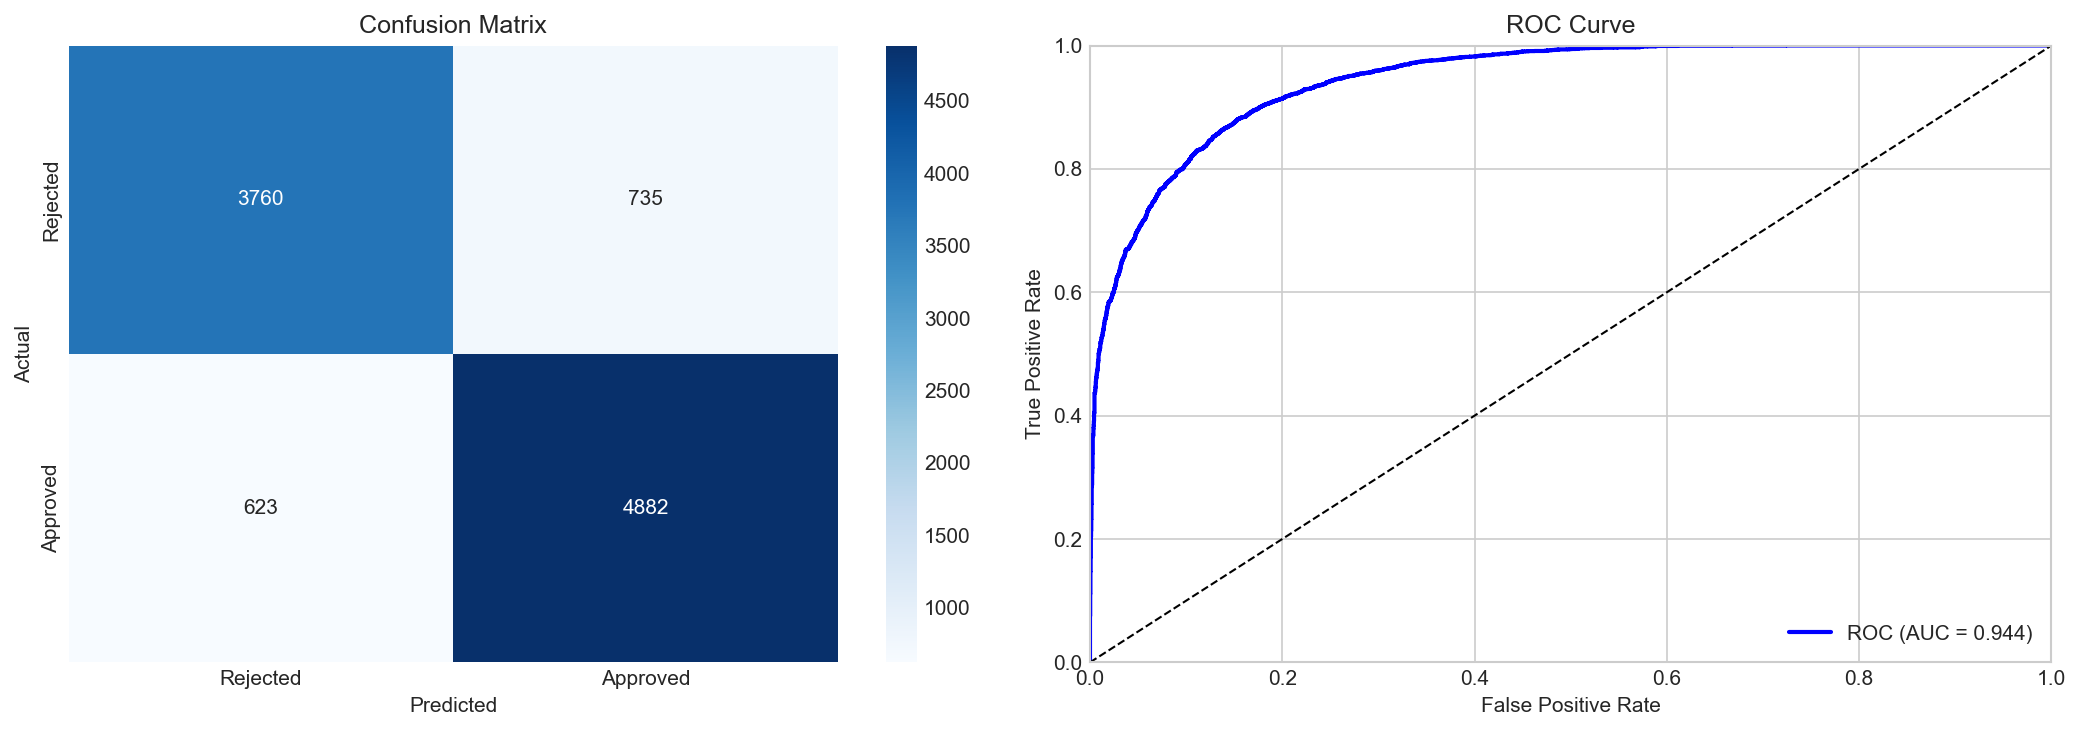
\includegraphics[width=\textwidth]{lr_evaluation.png}
    \caption{Logistic Regression: Confusion Matrix and ROC Curve}
    \label{fig:lr_eval}
\end{figure}

Confusion Matrix Analysis:
\begin{itemize}
    \item \textbf{True Negatives}: 3,760 (correctly rejected)
    \item \textbf{False Positives}: 735 (incorrectly approved)
    \item \textbf{False Negatives}: 623 (incorrectly rejected)
    \item \textbf{True Positives}: 4,882 (correctly approved)
\end{itemize}

\subsection{Feature Importance Analysis}

\begin{figure}[H]
    \centering
    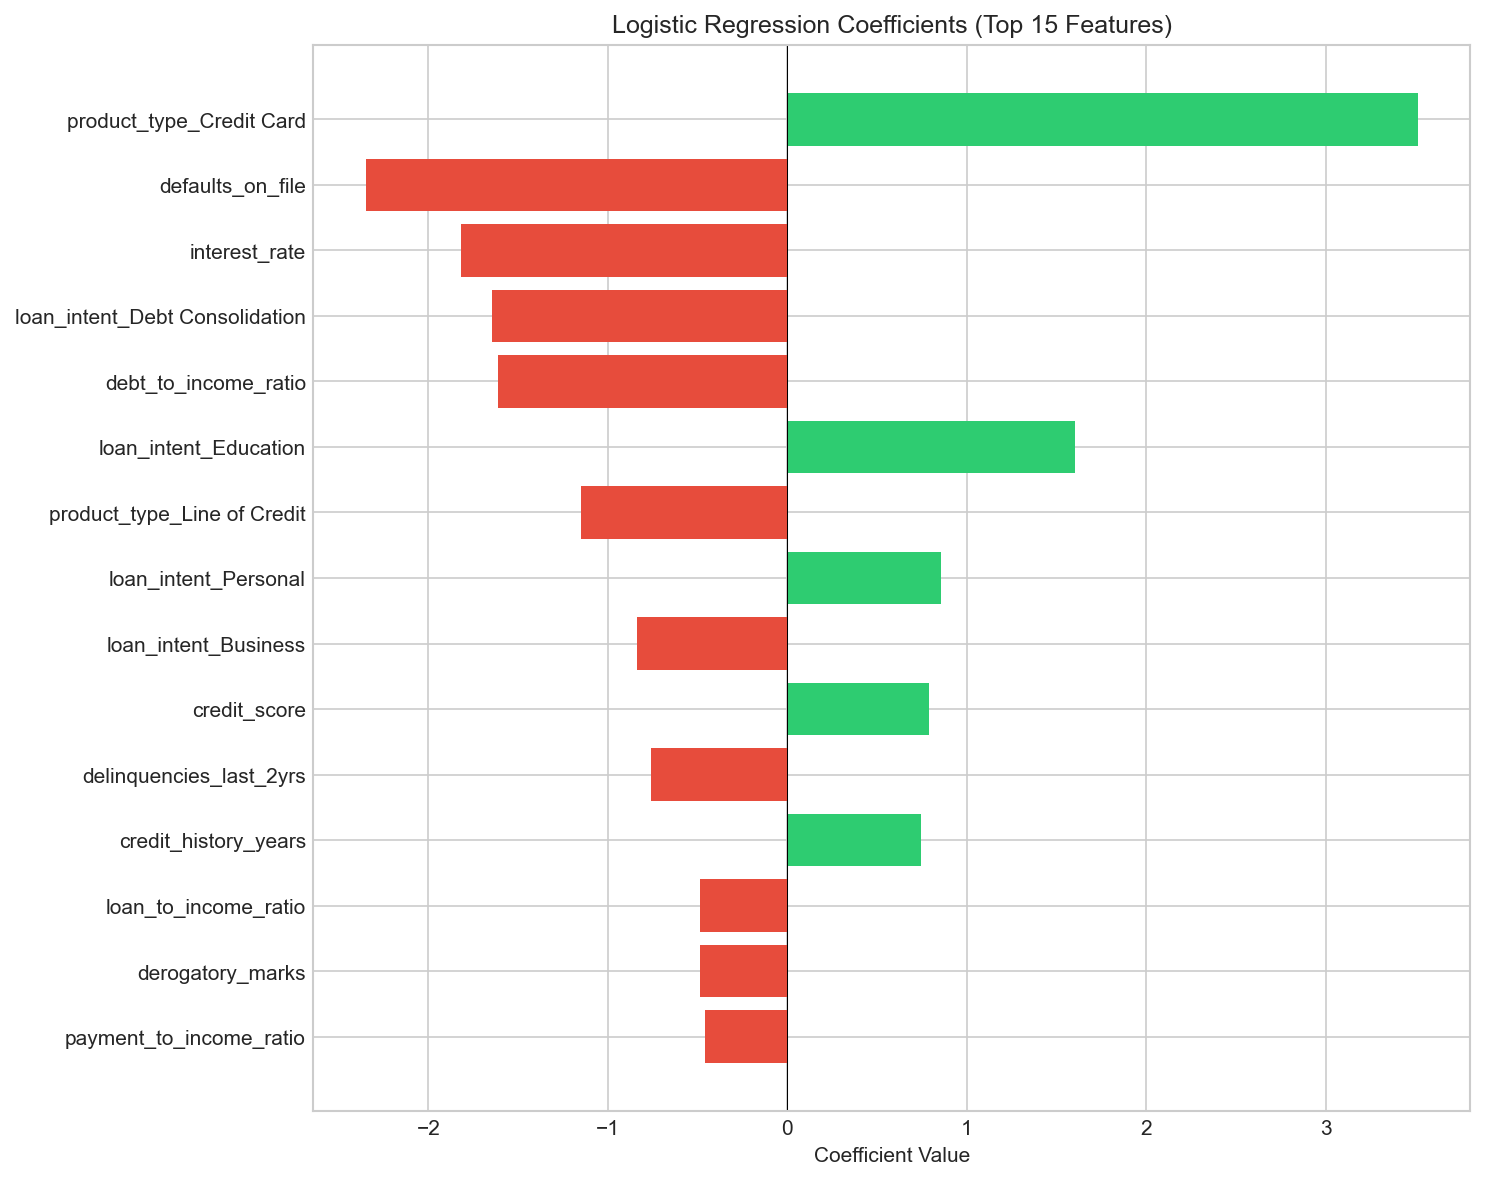
\includegraphics[width=0.9\textwidth]{lr_feature_importance.png}
    \caption{Logistic Regression Coefficients (Top 15 Features)}
    \label{fig:lr_importance}
\end{figure}

\subsubsection{Coefficient Interpretation}

For coefficient $\beta_i$, the odds ratio $e^{\beta_i}$ represents how much the odds of approval multiply per unit increase in the feature.

\begin{table}[H]
\centering
\caption{Top Features by Odds Ratio}
\begin{tabular}{lccp{6cm}}
\toprule
\textbf{Feature} & \textbf{Coef.} & \textbf{Odds Ratio} & \textbf{Interpretation} \\
\midrule
Credit Card & +3.51 & 33.5x & Credit card applicants are 33x more likely to be approved \\
Defaults on File & -2.35 & 0.095 & Having defaults reduces odds by 90\% \\
Interest Rate & -1.82 & 0.16 & Higher rates indicate 6x lower approval odds \\
Debt Consolidation & -1.65 & 0.19 & Debt consolidation loans 5x less likely approved \\
Education Loan & +1.60 & 4.96 & Education loans 5x more likely approved \\
Credit Score & +0.79 & 2.20 & 1 std increase $\rightarrow$ 2.2x odds \\
\bottomrule
\end{tabular}
\end{table}

\subsection{Key Insights}

\begin{enumerate}
    \item \textbf{Product Type Dominates}: Credit Card products have dramatically higher approval odds than Personal Loans or Lines of Credit.
    \item \textbf{Loan Intent Matters}: Education loans are favored; debt consolidation is penalized.
    \item \textbf{Credit History is Critical}: Defaults and delinquencies strongly reduce approval chances.
    \item \textbf{Linear Model Works}: 86\%+ accuracy suggests the problem is largely linearly separable.
\end{enumerate}

\subsection{Conclusion for Logistic Regression}

Logistic Regression provides a strong, interpretable baseline:
\begin{itemize}
    \item 86.42\% accuracy exceeds the 80\% threshold we set
    \item 94.39\% ROC-AUC indicates excellent discrimination
    \item Low CV variance ensures reliability
    \item Coefficients provide actionable business insights
\end{itemize}

\textbf{Next Steps}: We proceed to Decision Trees to test if threshold effects and feature interactions can improve upon this baseline.

\newpage

% Section 6: Conclusion (Placeholder)
\section{Summary and Next Steps}

\subsection{Work Completed}

\begin{enumerate}
    \item \textbf{Data Exploration}: Comprehensive EDA with 6 visualizations
    \item \textbf{Preprocessing}: Feature selection, encoding, scaling, and train-test split
    \item \textbf{Logistic Regression}: Complete implementation with hyperparameter tuning
\end{enumerate}

\subsection{Upcoming Work}

\begin{enumerate}
    \item Decision Tree and Random Forest models
    \item XGBoost implementation
    \item Deep Learning model with Keras
    \item Model comparison and selection
    \item Streamlit web application
    \item Deployment to Streamlit Cloud
\end{enumerate}

\newpage

% References
\section{References}

\begin{enumerate}
    \item Scikit-learn Documentation: \url{https://scikit-learn.org/}
    \item TensorFlow/Keras Documentation: \url{https://www.tensorflow.org/}
    \item Basel Committee on Banking Supervision. (2004). International Convergence of Capital Measurement and Capital Standards.
    \item Hastie, T., Tibshirani, R., \& Friedman, J. (2009). The Elements of Statistical Learning.
\end{enumerate}

\end{document}
